\section{Three-Level AC-Stark Shift of the \texorpdfstring{$f_{01}$}{f01} Resonance}
\label{sec:ac-stark-shift}

We calculate the change of the central $f_{01}$ resonance for a
$40~\mu\mathrm{s}$ constant square pulse and for $10~\mu\mathrm{s}$
root-Lorentzian and echo-root-Lorentzian spectroscopy pulses.  All calculations
use the conventional drive--qubit detuning
$\Delta=\omega_d-\omega_{01}$.  The simulation retains
$\{|g\rangle,|e\rangle,|f\rangle\}$, but $|f\rangle$ is used here as the
virtual transmon level that shifts $f_{01}$; the plotted observable is the
central excitation response $P_e+P_f$, not the position of the
$g\leftrightarrow f$ transition.  In this basis, the rotating-frame
Hamiltonian of Eq.~\eqref{eq:numerical-hamiltonian} is
\begin{equation}
    \frac{H(t)}{\hbar}=
    \begin{pmatrix}
        0 & \Omega(t)/2 & 0 \\
        \Omega(t)/2 & -\Delta & \Omega(t)/\sqrt{2} \\
        0 & \Omega(t)/\sqrt{2} & -2\Delta+\alpha
    \end{pmatrix},
    \label{eq:qutrit-ac-stark-hamiltonian}
\end{equation}
where $\alpha=\omega_{12}-\omega_{01}<0$.  For a constant drive, virtual
coupling between $|e\rangle$ and $|f\rangle$ gives the weak-drive result
\begin{equation}
    \delta f_{01}^{(\mathrm{const})}
    \equiv \frac{\Delta_{\mathrm{res}}}{2\pi}
    \simeq
    -\frac{(\Omega_0/2\pi)^2}
    {2(\alpha/2\pi)}.
    \label{eq:qutrit-ac-stark-shift}
\end{equation}
Because $\alpha<0$, the constant-pulse dressed $f_{01}$ resonance moves to
positive detuning.  The exact values reported below are obtained by
diagonalizing Eq.~\eqref{eq:qutrit-ac-stark-hamiltonian} at constant
$\Omega(t)=\Omega_0$ and minimizing the dressed $g$--$e$ gap.

For the shaped pulses, $\Omega(t)=\Omega_0 f(t)$ with the root-Lorentzian
envelope of Eq.~\eqref{eq:finite-generalized-lorentzian}, order $n=1/2$, and
endpoint amplitude $c=0.002$.  A useful weak-drive phase-average estimate is
\begin{equation}
    \delta f_{01}^{(\mathrm{shape})}
    \simeq
    -\frac{(\Omega_0/2\pi)^2}{2(\alpha/2\pi)}
    \left\langle f^2\right\rangle_t,
    \qquad
    \left\langle f^2\right\rangle_t
    =\frac{2\sigma}{L}\tan^{-1}\!\left(\frac{L}{2\sigma}\right),
    \label{eq:shaped-ac-stark-average}
\end{equation}
where
$\sigma=(L/2)/\sqrt{c^{-2}-1}=0.010000~\mu\mathrm{s}$ and
$\langle f^2\rangle_t=0.003138$.  The echo phase inversion changes
$f(t)\rightarrow-f(t)$ in the second half and therefore does not reverse this
quadratic Stark term.  Consequently, the root-Lorentzian and
echo-root-Lorentzian pulses have the same leading phase-average estimate.

The experimentally visible feature of a finite pulse need not coincide with
Eq.~\eqref{eq:shaped-ac-stark-average}, because the final population also
contains coherent finite-pulse interference.  We therefore report both
quantities.  For the ordinary root-Lorentzian pulse, the operational center is
the local maximum of $P_e+P_f$ within
$|\Delta|/(2\pi)\leq0.5~\mathrm{MHz}$.  For the echo-root-Lorentzian pulse it
is the corresponding central minimum.  The spectra are evaluated on a
$0.05~\mathrm{MHz}$ grid and the extrema are refined with cubic interpolation.
The central-feature extraction is shown for
$\Omega_0/(2\pi)\geq20~\mathrm{MHz}$, where the feature has sufficient
contrast.

\begin{table}[b]
    \caption{Calculated displacement of the $f_{01}$ resonance or central
    finite-pulse feature, in MHz.  The shaped phase average is common to the
    two Lorentzian-derived envelopes.}
    \label{tab:ac-stark-f01-shifts}
    \begin{ruledtabular}
    \begin{tabular}{ccccc}
        $\Omega_0/(2\pi)$ &
        \multicolumn{1}{c}{Constant dressed} &
        \multicolumn{1}{c}{Root maximum} &
        \multicolumn{1}{c}{Echo-root minimum} &
        \multicolumn{1}{c}{Shaped phase average} \\
        \colrule
        20 & 0.980 & 0.002 & 0.003 & 0.003 \\
        40 & 3.685 & -0.001 & -0.002 & 0.013 \\
        60 & 7.605 & 0.079 & -0.013 & 0.028
    \end{tabular}
    \end{ruledtabular}
\end{table}

The small negative position of the echo-root minimum at the largest drive is
an operational finite-pulse feature position, not a negative instantaneous
AC-Stark shift.  It results from the interference defining the echo spectrum.
The phase-average Stark term remains positive for both shaped protocols.

The time-domain maps solve the three-level Lindblad equation with
$T_1=51.24~\mu\mathrm{s}$, $T_\phi=7.87~\mu\mathrm{s}$, an initial
$|g\rangle$ state, 31 peak Rabi frequencies from 0 to $60~\mathrm{MHz}$, and
101 detuning points over the full $100~\mathrm{MHz}$ domain, from
$-50$ to $50~\mathrm{MHz}$.  Additional 401-point scans resolve the central
$20~\mathrm{MHz}$ span and the $1~\mathrm{MHz}$ Lorentzian zooms in
Figs.~\ref{fig:ac-stark-domains} and \ref{fig:ac-stark-f01-zoom}.  The model
uses the rotating-wave approximation, so it does not include a
counter-rotating Bloch--Siegert shift.

\begin{figure}[t]
    \centering
    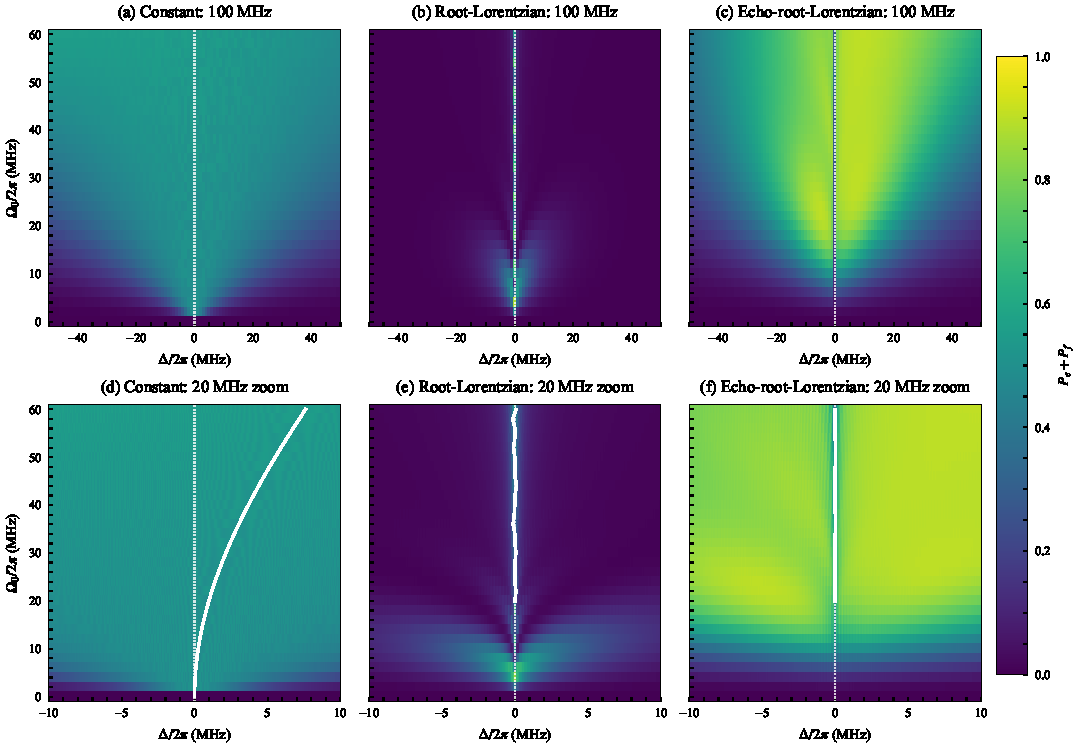
\includegraphics[width=0.98\textwidth]{../figures/paper/11_ac_stark_qutrit_10us.pdf}
    \caption{Full-domain and central-zoom three-level calculations of the
    $f_{01}$ response for a
    $40~\mu\mathrm{s}$ constant pulse and $10~\mu\mathrm{s}$ shaped pulses.
    (a)--(c) Final excitation $P_e+P_f$ over the full
    $-50$ to $50~\mathrm{MHz}$ domain for constant, root-Lorentzian, and
    echo-root-Lorentzian drives.  (d)--(f) Corresponding $20~\mathrm{MHz}$
    zooms from $-10$ to $10~\mathrm{MHz}$.  The dotted line is the bare
    $f_{01}$ frequency.  In the zooms, the solid lines show the
    exact constant-drive dressed center, the root-Lorentzian local maximum,
    and the echo-root-Lorentzian central minimum, respectively; shaped-pulse
    centers are omitted below $20~\mathrm{MHz}$ peak Rabi frequency where the
    local-extremum definition is not robust.}
    \label{fig:ac-stark-domains}
\end{figure}

\begin{figure}[t]
    \centering
    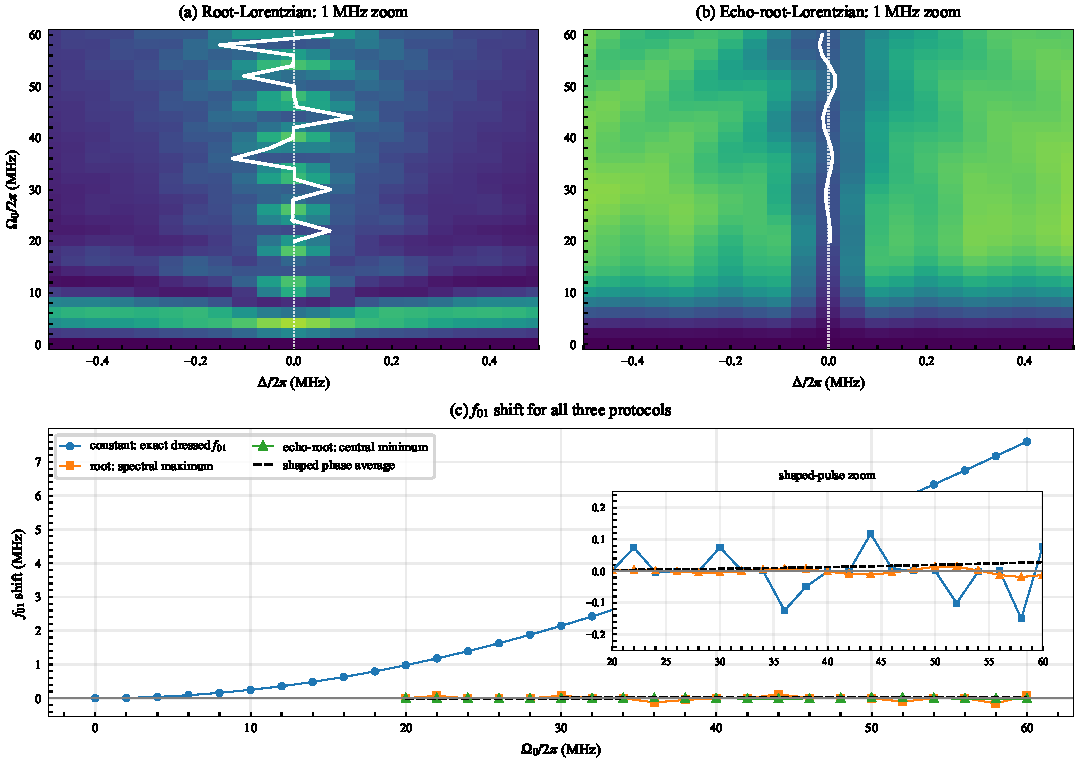
\includegraphics[
        width=0.98\textwidth,
        trim=0 176bp 0 0,
        clip
    ]{../figures/paper/12_ac_stark_f01_zoom_shift.pdf}
    \caption{Fine $f_{01}$ comparison for the Lorentzian-derived pulses.
    (a),(b) One-megahertz central zooms of the
    root-Lorentzian and echo-root-Lorentzian final excitation, respectively.
    The dotted line marks the bare $f_{01}$ frequency and the solid lines mark
    the extracted maximum or central minimum.}
    \label{fig:ac-stark-f01-zoom}
\end{figure}
\FloatBarrier

\subsection{Measured resonance-center stability}

The AC-Stark calculation above predicts a clear separation between the
instantaneous shift produced by a constant drive and that produced by the
Lorentzian-derived envelopes.  At the upper edge of the experimentally
selected operating window,
$\Omega_0/(2\pi)=8.973~\mathrm{MHz}$, the weak-drive constant-pulse estimate
from Eq.~\eqref{eq:qutrit-ac-stark-shift} is approximately
$0.20~\mathrm{MHz}$.  Multiplication by the shaped-pulse factor
$\langle f^2\rangle_t=0.003138$ reduces the phase-average estimate to
$0.63~\mathrm{kHz}$.  The wider-range three-level calculation in
Figure~4 of the Letter confirms this separation over the wider calculated
drive range.  The echo phase
inversion does not cancel the quadratic Stark term; rather, the small
time-averaged squared envelope suppresses it, while finite-pulse interference
determines the experimentally visible central minimum.

We test the corresponding center stability directly in the q1
amplitude-sweep data used in
Figs.~\ref{fig:amplitude-robustness-2d}--\ref{fig:amplitude-resolution-metrics}.
Each amplitude slice is fit with the same Gaussian dip estimator and
preprocessing described in Sec.~\ref{sec:data-analysis}.  To avoid selecting
the result being tested, the center-quality mask uses only finite fit
parameters, contrast $A\geq0.02$, and FWHM
$\Gamma_f\leq0.12~\mathrm{MHz}$; it does not impose the usual
$|\delta_0|\leq0.050~\mathrm{MHz}$ center gate.  We then restrict the summary
to the independently selected matched-simulation operating window
$\Omega_0/(2\pi)=2.475$--$8.973~\mathrm{MHz}$, defined by $Q\geq0.10$.

The inverse-variance weighted center is
$\overline{\delta_0}=-0.47\pm0.15~\mathrm{kHz}$, where the stated uncertainty
uses the fit covariance only.  Relative to this center, the 42 retained
amplitude slices have an empirical RMS displacement of $3.02~\mathrm{kHz}$
and a maximum absolute displacement of $7.47~\mathrm{kHz}$.  The constant-fit
value $\chi_\nu^2=9.94$ shows that the slice-to-slice scatter is larger than the
local covariance errors; the measurements therefore do not establish strict
statistical constancy.  Instead, the RMS and maximum excursion quantify the
practical center stability, including fit variation, slow experimental drift,
and any residual finite-pulse or AC-Stark contribution.  The observed
few-kilohertz, nonmonotonic excursions are nevertheless far smaller than the
approximately $0.20~\mathrm{MHz}$ constant-drive Stark displacement expected
at the same upper peak Rabi frequency.

\begin{figure}[t]
    \centering
    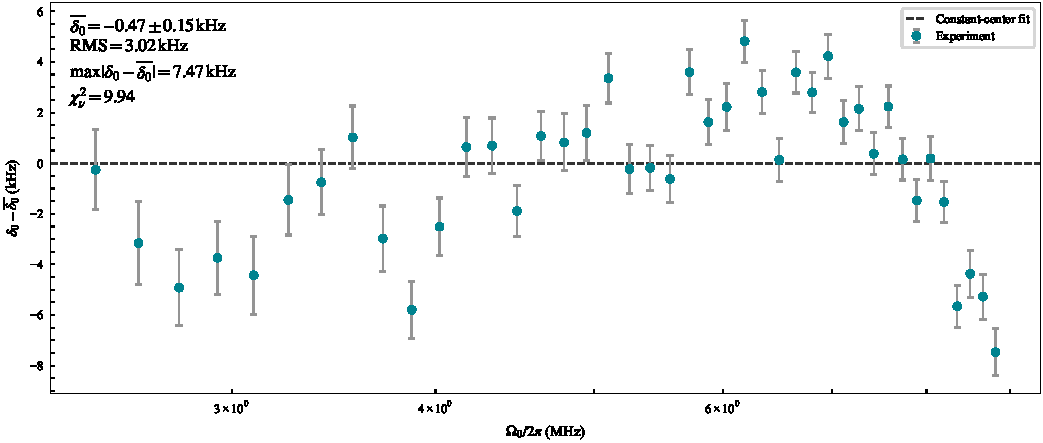
\includegraphics[width=0.98\textwidth]{../figures/paper/03_amplitude_center_stability.pdf}
    \caption{Measured resonance-center stability across the independently
    selected q1 echo--root--Lorentzian operating window.  Points show the
    fitted center displacement relative to the inverse-variance weighted mean;
    vertical bars are one-standard-deviation covariance uncertainties.  The
    dashed line is the weighted mean and the gray band spans the empirical RMS
    displacement of $\pm3.02~\mathrm{kHz}$.  The maximum absolute displacement
    is $7.47~\mathrm{kHz}$.  No center-position gate is used to select the
    displayed points.  Although $\chi_\nu^2=9.94$ rules out interpreting the
    covariance errors as a complete noise model, the bounded center excursion
    directly quantifies amplitude robustness and is strongly separated from
    the constant-drive AC-Stark displacement in
    Fig.~4 of the Letter.}
    \label{fig:measured-center-stability}
\end{figure}

\subsection{Three-level optimization of resonance-center stability}
\label{subsec:drag-stark-optimization}

We further test whether a derivative quadrature and a dynamic frequency
correction can stabilize the central echo-root-Lorentzian feature in the
three-level model.  The reproducible calculation is contained in
\path{notebooks/paper/34_drag_echo_lorentzian_qutrit.ipynb}.  It uses a
$10~\mu\mathrm{s}$ pulse with $c=0.002$, echo inversion enabled,
$\alpha/(2\pi)=-200~\mathrm{MHz}$,
$T_1=51.24~\mu\mathrm{s}$, and $T_\phi=7.87~\mu\mathrm{s}$.  The final
populations $P_g$, $P_e$, and $P_f$ are calculated over peak Rabi frequencies
from 0 to $80~\mathrm{MHz}$ and detunings from $-1$ to $1~\mathrm{MHz}$.

The complex drive is written as $\Omega_I-i\Omega_Q$.  Its derivative
quadrature is
\begin{equation}
    \Omega_Q(t)
    =-\frac{\beta}{\alpha}\frac{d\Omega_I(t)}{dt},
    \label{eq:echo-drag-quadrature}
\end{equation}
where the derivative acts on the smooth positive envelope within each half
of the pulse and the same $0/\pi$ echo phase is applied to both quadratures.
The ideal instantaneous phase jump itself is not differentiated.  We use the
moderate value $\beta=2$, for which the peak quadrature is $6.11\%$ of the
peak in-phase drive.  In addition, the instantaneous drive detuning is
corrected according to
\begin{equation}
    \frac{\Delta_{\mathrm{corr}}(t)}{2\pi}
    =\kappa
      \left[\frac{\Omega_I(t)}{2\pi}\right]^2,
    \label{eq:optimized-stark-compensation}
\end{equation}
with $\kappa$ expressed in $\mathrm{MHz}^{-1}$.  This is equivalent to a phase
chirp satisfying $\dot{\phi}(t)=-\Delta_{\mathrm{corr}}(t)$, up to the stated
detuning convention.

For each candidate $\kappa$, the notebook calculates a compact map over
$\Omega_0/(2\pi)=20$--$80~\mathrm{MHz}$.  The central minimum of $P_e$ is
identified within $|\Delta|/(2\pi)\leq0.35~\mathrm{MHz}$ and refined with a
local quadratic fit.  The optimization target is its RMS displacement from
the bare transition,
\begin{equation}
    \mathcal{L}
    =\sqrt{\left\langle\delta_0^2(\Omega_0)\right\rangle_{\Omega_0}},
    \label{eq:stark-optimization-cost}
\end{equation}
while the maximum $P_f$ is retained as an independent leakage diagnostic.  A
coarse scan over $\kappa=-0.005$ to $0.005~\mathrm{MHz}^{-1}$ is followed by a
fine scan around the best coarse value.  As shown in
Fig.~\ref{fig:drag-stark-optimization}(a), the optimum for this model is
\begin{equation}
    \kappa=+0.001750~\mathrm{MHz}^{-1}.
\end{equation}
The fitted central minimum then has an RMS displacement of $3.54~\mathrm{kHz}$
from the bare transition and a maximum absolute displacement of
$6.60~\mathrm{kHz}$ over the optimization amplitudes.  These values are
simulation results, not experimentally calibrated correction parameters.

The full-resolution comparison is shown in
Fig.~\ref{fig:drag-stark-optimization}(b).  Relative to the uncorrected
echo-root-Lorentzian calculation, the combined DRAG and Stark-corrected pulse
reduces the maximum $P_f$ from $0.1781$ to $0.1598$.  Over
$\Omega_0/(2\pi)=40$--$80~\mathrm{MHz}$, the mean $P_f$ decreases from
$0.0669$ to $0.0614$.  The low-amplitude population response retains some
coherent oscillatory structure: the optimization in
Eq.~\eqref{eq:stark-optimization-cost} constrains the resonance position and
does not explicitly minimize population ripple.  Thus the result demonstrates
improved center stability and leakage within the model, but not complete
removal of all finite-pulse oscillations.

\begin{figure}[p]
    \centering
    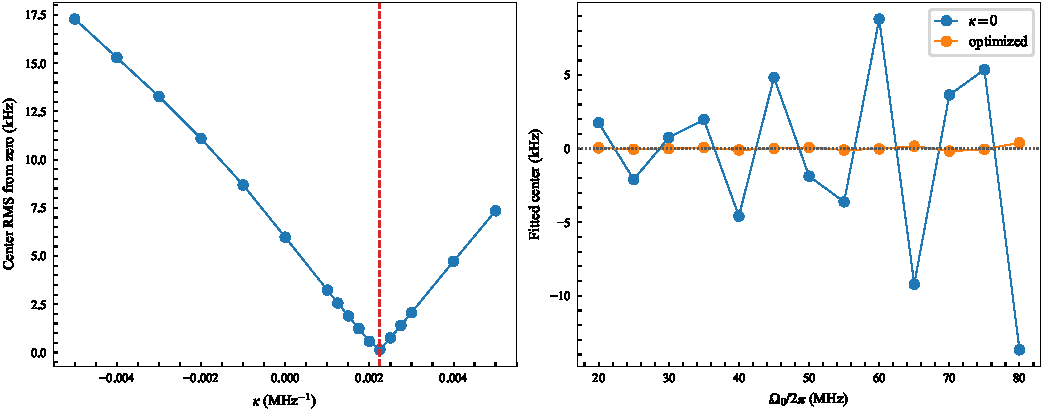
\includegraphics[width=0.98\textwidth]{../figures/paper/15_stark_kappa_optimization_80mhz.pdf}
    \par\vspace{0.8em}
    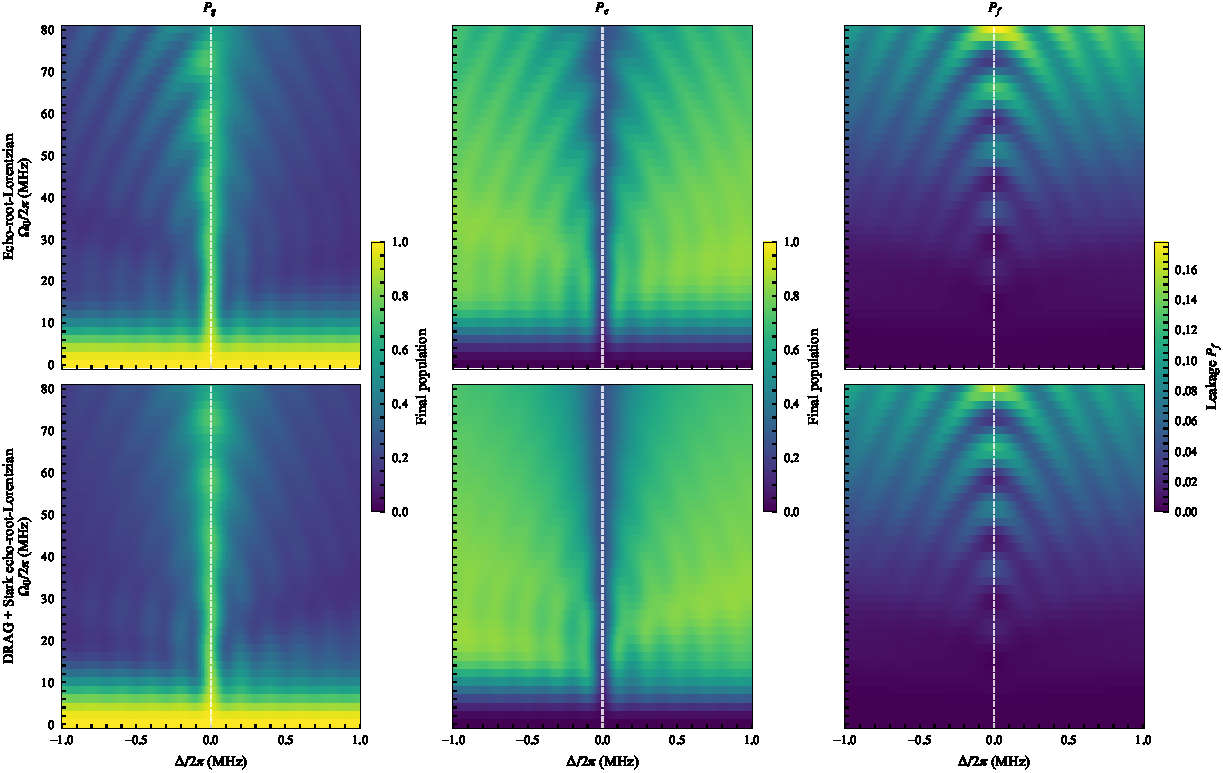
\includegraphics[width=0.98\textwidth]{../figures/paper/13_drag_echo_lorentzian_qutrit_80mhz.pdf}
    \caption{Three-level optimization of the echo-root-Lorentzian response.
    (a) Quadratic Stark-correction scan.  The left panel shows the RMS
    fitted-center displacement from the bare transition versus $\kappa$; the
    dashed line marks the selected coefficient.  The right panel compares the
    fitted central minimum without the correction and at the optimized value.
    (b) Full $-1$ to $1~\mathrm{MHz}$ detuning maps.  The upper row is the
    original echo pulse and the lower row includes the $\beta=2$ derivative
    quadrature and optimized quadratic Stark correction.  Columns show
    $P_g$, $P_e$, and $P_f$; dashed lines mark the bare transition.}
    \label{fig:drag-stark-optimization}
\end{figure}

\FloatBarrier
